
%Chapter 2

\renewcommand{\thechapter}{2}

\chapter{The LUX Detector}

\section{Introduction}

The LUX experiment is located 4850 ft underground (4300 m w.e.) at the Sanford Underground Research Facility in Lead, South Dakota. After running for 85.3 live days in 2013, LUX has recently set the most sensitive limit for a spin independent WIMP scattering cross section [ref] and is expected to achieve five times the sensitivity after a 300 day run ending in 2015. Nobel elements are ideal candidates for WIMP detection, they are easy to purify and are transparent to their own scintillation light. Xenon is especially favorable do to it's  large atomic mass (131.3 amu) and high liquid phase density ($\rm \sim$2.9 kg/l) which provides both an excellent target for coherent WIMP scattering while simultaneously providing excellent shielding from external radioactivity. Xenon also radio pure with established techniques to remove and monitor the residual, troublesome radio isotopes of argon and krypton found in the atmosphere from which the xenon is distilled [refs]. 
WIMPs being electrically neutral would primarily interact with the xenon target nuclei producing nuclear recoils (NR) whereas typical backgrounds in the detector, gammas and betas, interact with the electrons producing electronic recoils (ER). In liquid xenon ER events can be further discriminated from NR events by about a factor of 1000 by taking the charge to light ratio of the interaction.



\section{The LUX TPC}

The LUX detector is a two phase xenon time projection chamber TPC,  [ref LUX inst]. . The detector contains two PMT arrays on the top and bottom with 61 PMTs each for a total of 122 PMTs, with quantum efficiencies ranging from 30-40\%. The active region consists of a 49 cm length between the cathode and gate grid with a 47 cm diameter of the dodecagonal geometry. The drift field between the cathode and gate is 180 V/cm resulting in an electron drift velocity of 1.51 mm/$\rm \mu s$. The liquid level terminates 5-6mm above the gate grid as the liquid xenon spills over into a weir reservoir. The anode grid is placed 1.0 cm above the gate grid and used to bias the extraction field of 6 [kV/cm] where electrons are removed from the liquid and accelerated causing electroluminescence in the gas phase.  LUX contains a gross 350 kg of xenon of which 250 kg are in the active region and 118 kg fiducial.  The detector in shown in figures \ref{fig:LUX_Real}, \ref{fig:LUX_Davis} and \ref{fig:LUX_TPC}.

 \begin{figure}[h!]\centering
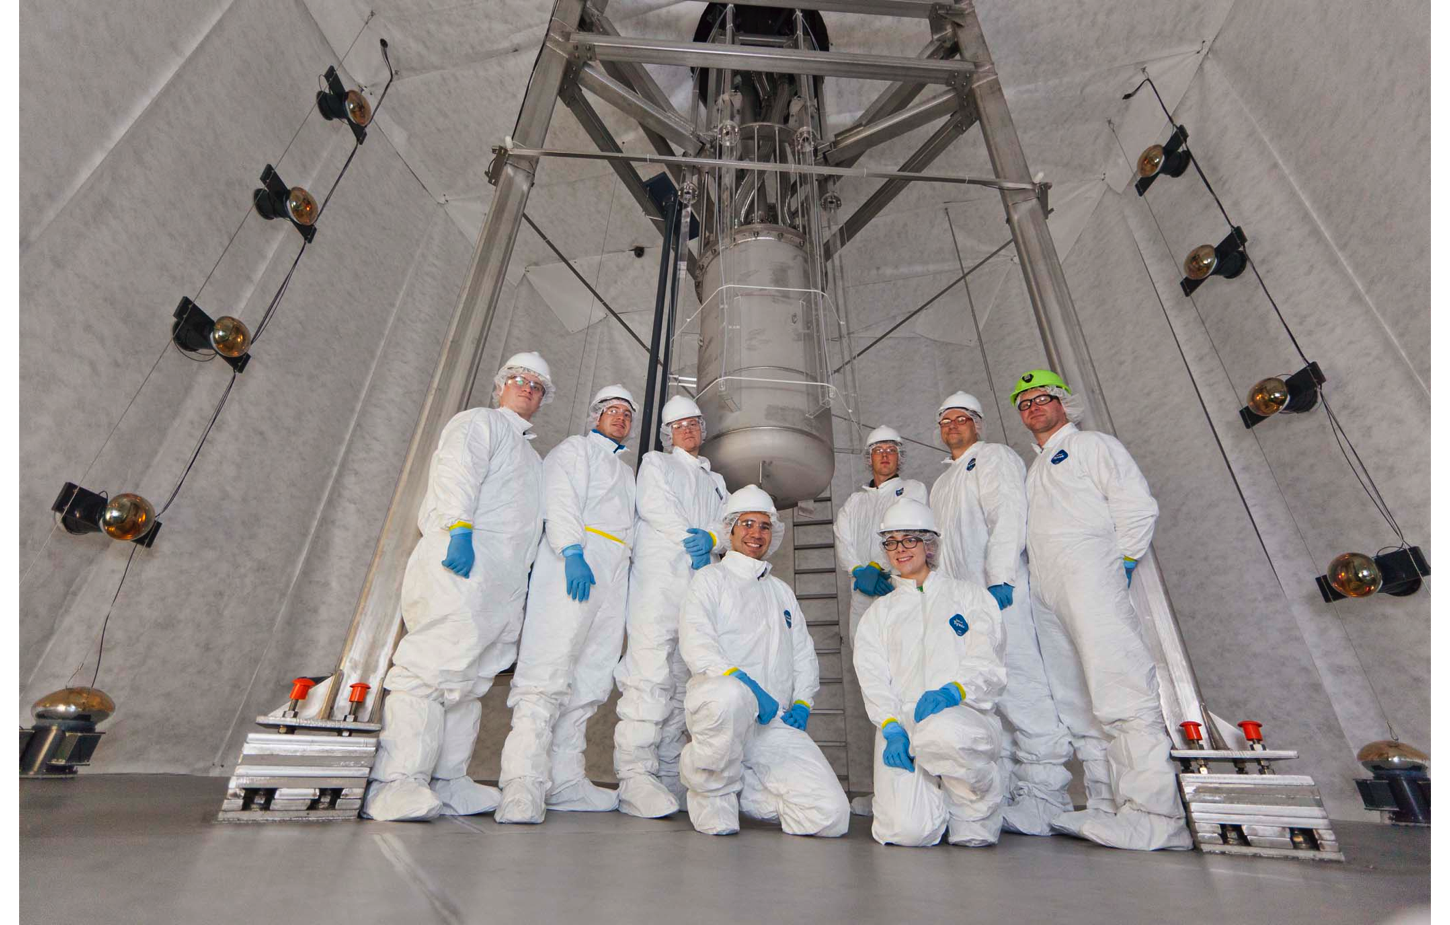
\includegraphics[scale=0.5]{Chapter_LUX_Det/LUX_Real.png}
\caption{Photo of the LUX detector and the surrounding water tank.}
\label{fig:LUX_Real}
\end{figure}

\begin{figure}[h!]\centering
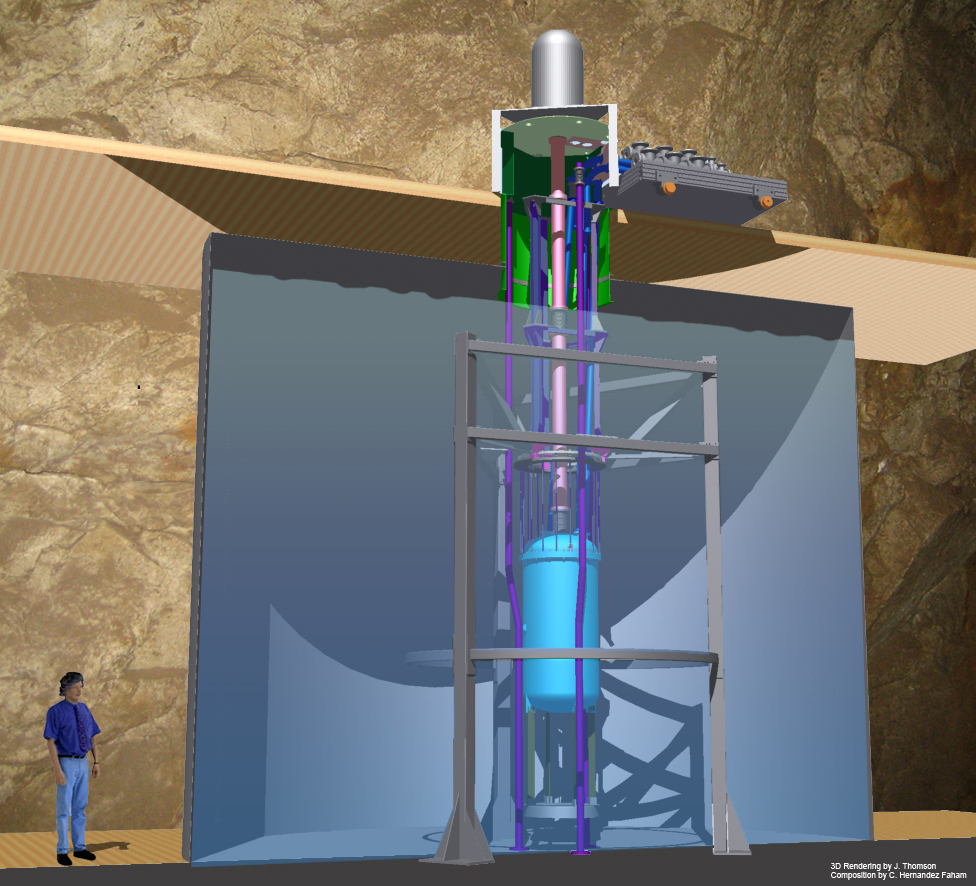
\includegraphics[scale=0.35]{Chapter_LUX_Det/Davis_3D_tank.jpg}
\caption{Schematic of the LUX detector and the surrounding water tank.}
\label{fig:LUX_Davis}
\end{figure}

 \begin{figure}[h!]\centering
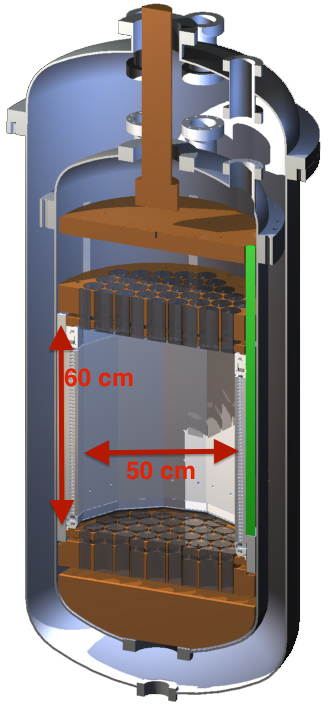
\includegraphics[scale=0.5]{Chapter_LUX_Det/LUX_half_rendering_white.jpg}
\caption{Illustration of the LUX detector's internals. The detector contains two arrays of PMTs on the top and bottom housing 61 PMTs each. Teflon panels on the edges of the active region are used to reflect scintillation signals. The vertical distance between the two PMT arrays is 60 cm, and the diameter to the outer edge of the teflon panels is 50 cm. }
\label{fig:LUX_TPC}
\end{figure}

%Add self shielding plot... 5 orders of magnitude reduction in the center.


\section{The Light and Charge Signals}

When energy is deposited in the active region of the xenon TPC it is converted to excitation, ionization and heat, equation \ref{eq:E_Q}. For a given energy deposit, NR events lose a significant portion of energy to heat leaving less energy available for excitation and ionization than an ER event. Xenon excitons de-excite on the order of nano seconds producing 175nm VUV scintillation light, recombining ion electron pairs also emit scintillation light. The two channels for photon production overlap in time and sum to produce the primary scintillation signal (S1), arriving within 10s of ns as the photons are collected by the  PMT arrays. Electrons which escape recombination with their ion pair feel the drift field and begin to drift upwards towards the gas phase (drift times of 0-324 $\rm \mu s$). Once extracted into the gas the electrons accelerate and electroluminece  producing a much larger secondary scintillation signal (S2), proportional the the number of electrons extracted. A schematic of an NR and ER event is shown in figures \ref{fig:TomS_ER} and figure \ref{fig:TomS_NR}. An illustration of an energy deposition in the LUX detector is show in figure \ref{fig:LUX_Event}. The timing separation between the S1 and S2 pulse is used to define the drift time and the hit pattern of the S2 signal on the top PMT array is used to define the XY position of the event. From the S1 and S2 signals the full x,y,z position and energy deposit of the event can be reconstructed.

%Show prompt fraction plot to describe event selection.


\begin{equation}
\begin{split}
\rm E= W\times n_q + Heat \\
\rm E= W (n_i + n_{ex}) + Heat \\
\rm E= W (n_\gamma + n_e) + Heat \\
\label{eq:E_Q}
\end{split}
\end{equation}

Where E is the energy of the deposit in keV, $\rm n_q$ is number of quanta (photons + electrons), $\rm n_i$, $\rm n_{ex}$, $\rm n_\gamma$ and $\rm n_e$ represent the number of ions, exitons, photons and electrons respectively. W for xenon has been measured to be 13.7 $\rm \pm$ 0.2  [quanta/eV] (refs).

 \begin{figure}[h!]\centering
 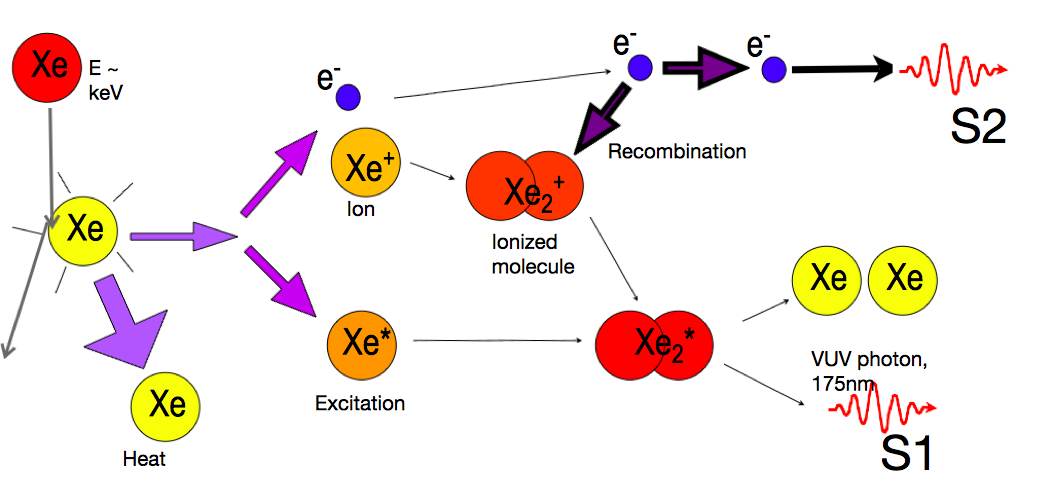
\includegraphics[width=150mm]{Chapter_LUX_Det/NR_T_Shutt.png}
\caption{Nuclear recoil (NR) event in xenon.}
\label{fig:TomS_ER}
\end{figure}

 \begin{figure}[h!]\centering
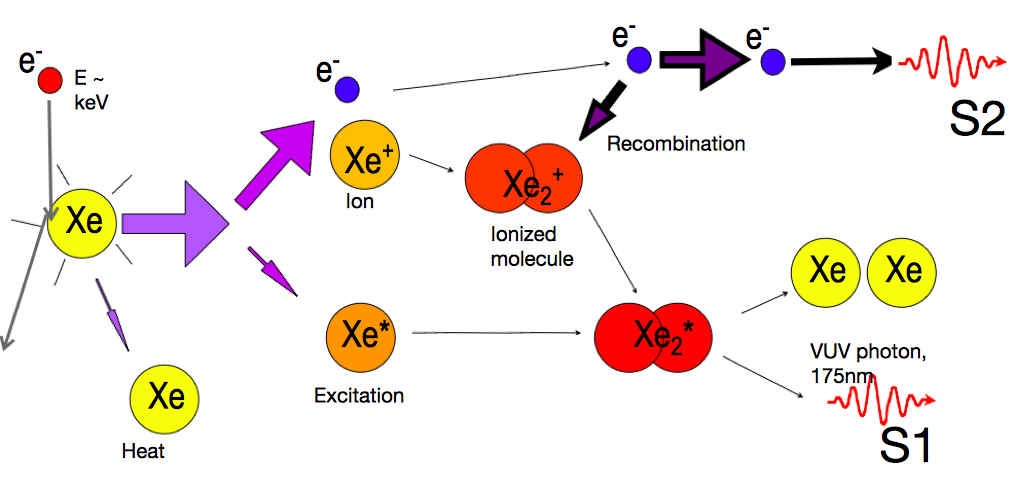
\includegraphics[width=150mm]{Chapter_LUX_Det/ER_T_Shutt.png}
\caption{Electronic recoil (ER) event in xenon}
\label{fig:TomS_NR}
\end{figure}

 \begin{figure}[h!]\centering
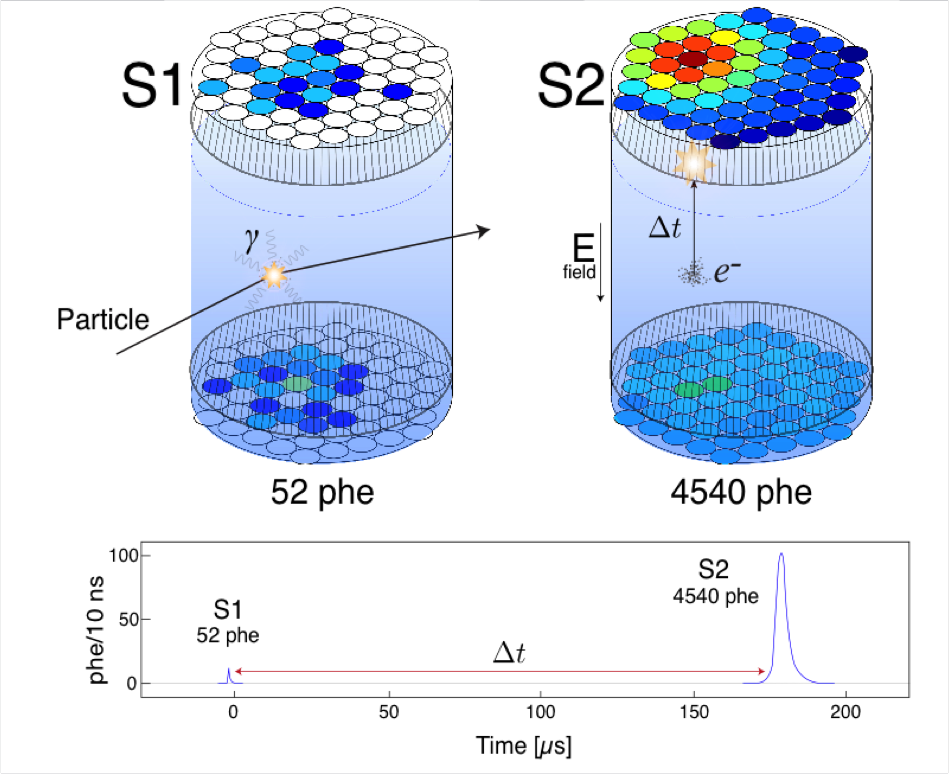
\includegraphics[width=150mm]{Chapter_LUX_Det/LUX_Event_Diagram.png}
\caption{Event diagram.}
\label{fig:LUX_Event}
\end{figure}

\section{Identifying S1, S2}
The primary and secondary signals have unique properties which can be used to identify their populations. The S1 signal is a fast spike summed along the PMT arrays, the signal decays in 10s of nano seconds as the primary scintillation and recombining electron ion pairs emit photons VUV (175nm). The S2 signal arrives several $\rm \mu s$ later with the electron population spread out about the centroid of the interaction due to diffusion. The characteristic S2 signal is one with a slow rise and corresponding slow fall, resembling a bell curve. A 2 keV event as seen by all 122 PMT channels is showing in figure \ref{fig:LUX_Golden}, the S1 pulse is spiked as the photons arrive and the S2 pulse is much larger with a slower rise-time  (the S2 pulse is larger since a single electron creates hundred of photons as it is accelerated in the extraction region). 

%Show prompt fraction plot to describe event selection.

 \begin{figure}[h!]\centering
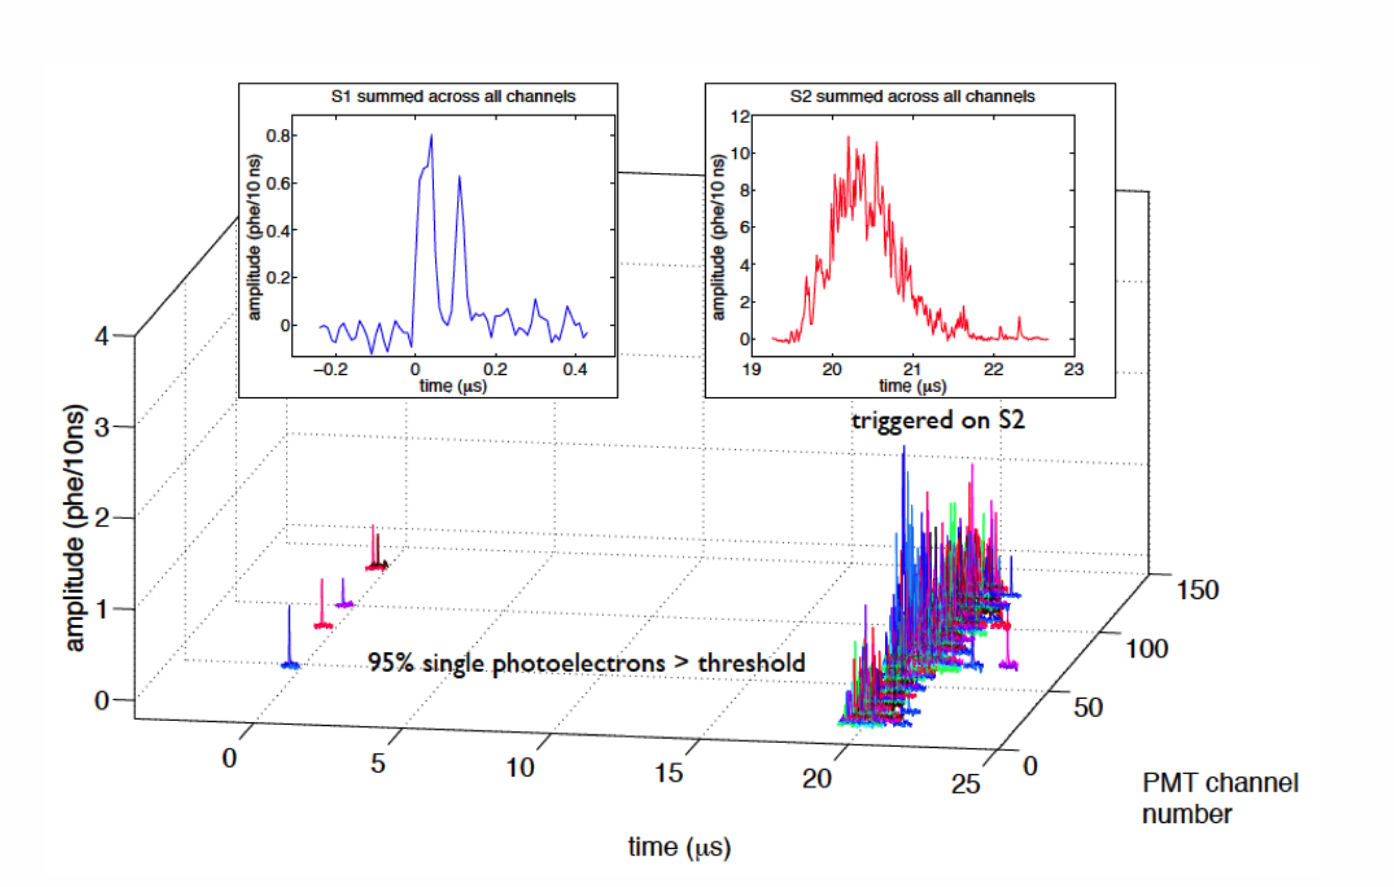
\includegraphics[width=130mm]{Chapter_LUX_Det/LUX_Golden_Event_2keV.png}
\caption{ 2keV ER event as seen by each PMT channel of the LUX detector. The S1 signal summed across all channels is overlaid on the top left, and the S2 signal summed across all channels is overlaid on the top right.}
\label{fig:LUX_Golden}
\end{figure}

We define a variable Prompt Fraction as the area covered in the first 10\% of the pulse normalized to the total area, and use it to identify S1 and S2 populations. For S1s this value will approach 1 and for S2s the value will be below 0.1, this provides for a figure of merit used to separation of the populations. The separation of population density is shown in figure \ref{fig:Prompt_Fraction} for the case of a $\rm ^{83m}Kr$ data set (41.5 keV gamma) and a tritium calibration data set (1-18.5 keV beta decay). The population of single electrons, single photons and the S1 S2 pairs associated with gammas, betas and alpha interactions are clearly visible and well separated when plotting the prompt  fraction variable vs. pulse area (PE). For the WIMP search we define `Golden' events consisting of single scatters with a single S1 paired with a subsequent S2 pulse, with this requirement each golden event has a well defined x,y coordinate and z making it possible to correct the signals for geometry and electron attenuation.

 \begin{figure}[h!]\centering
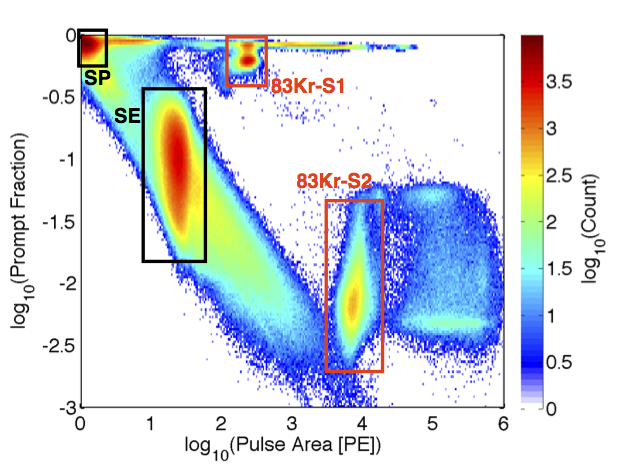
\includegraphics[width=110mm]{Chapter_LUX_Det/Kr_83_Density_text.png}
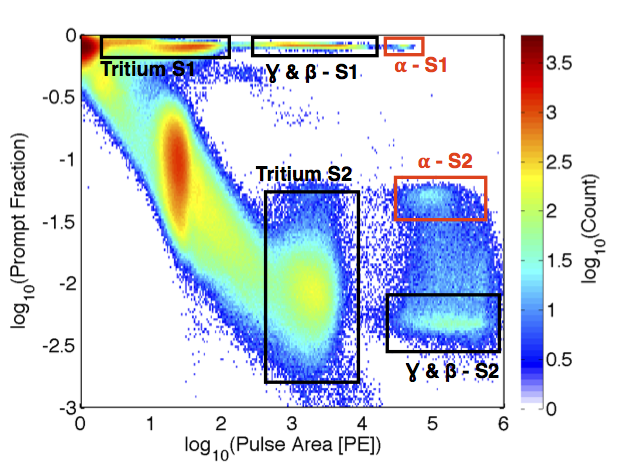
\includegraphics[width=110mm]{Chapter_LUX_Det/T_Density_text.png}
\caption{Density plot of prompt fraction vs. Pulse Area. Top: $\rm^{83m}Kr$ data set. Bottom: Tritium data set. Populations of single electrons, single photons and the S1 S2 pairs associated with gammas, betas and alpha are highlighted as rectangles.}
\label{fig:Prompt_Fraction}
\end{figure}


\section{LUX Science Result (WIMP limit)}

The first science run of the LUX detector consisted of 85.3 live days from April 21, 2013 to Aug 8, 2013. All single scatter (golden) events during the first science run are shown in figure \ref{fig:LUX_Result_Event}, with the vast majority of events occurring at the edges of the detector. For the WIMP search a fiducial cut is applied that reduces residual radioactivity from the detector surface and PMTs by another four orders of magnitude, thanks to the excellent self shielding properties of liquid xenon. The fiducial cut consists of a radial cut at radius less than 18 cm and a z cut of drift time between 38 and 305 $\rm \mu s$, the fiducial cut is shown in the figure.

 \begin{figure}[h!]\centering
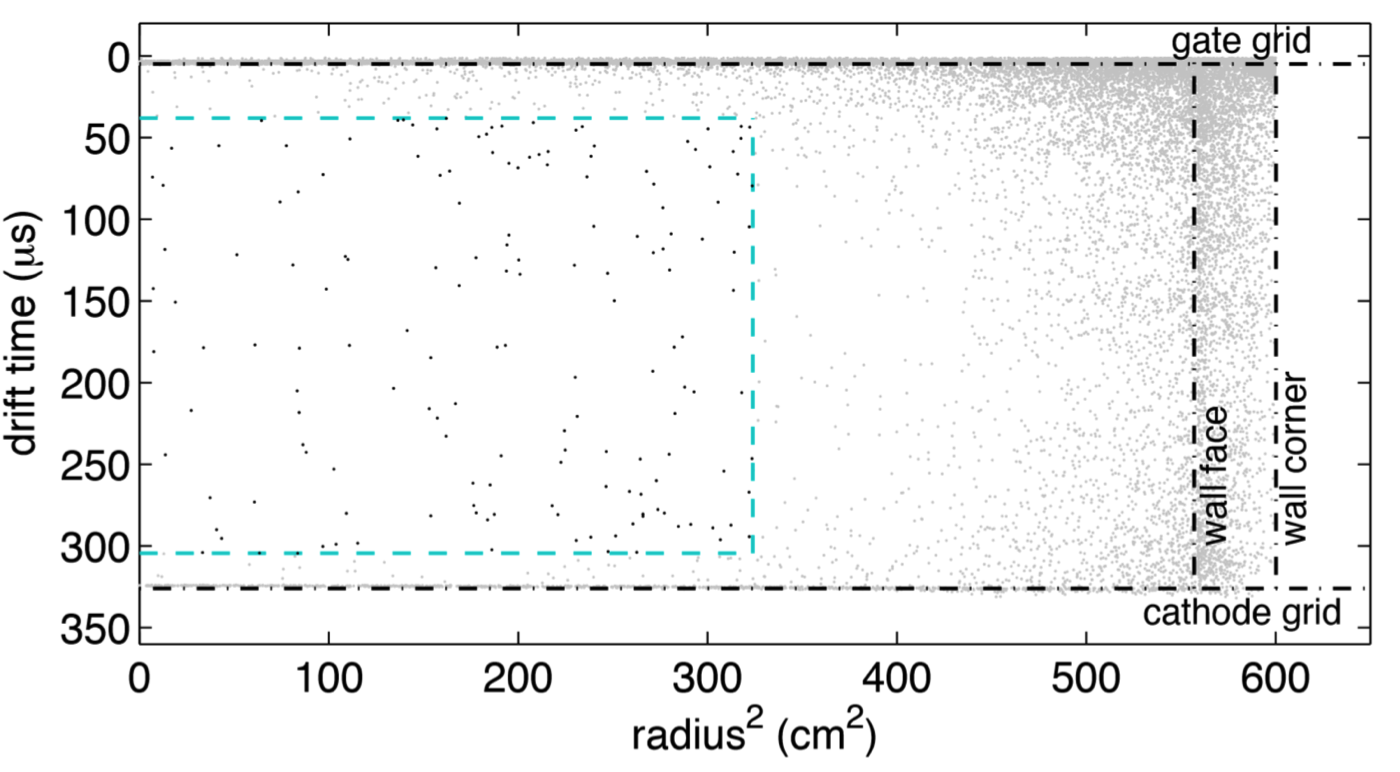
\includegraphics[width=120mm]{Chapter_LUX_Det/LUX_Result_Event.png}
\caption{All single scatter events seen in the active region of the LUX detector over the course of the first science run. The rectangular cut indicates the fiducial volume, in which the background rate is suppressed by another four orders of magnitude due xenon self shielding.}
\label{fig:LUX_Result_Event}
\end{figure}


Within the fiducial volume 160 events remain which meet our WIMP search energy requirement. The energy cut is placed in terms of S1 from 2-30 PE, corresponding to roughly 1.0 to 6 $\rm keV_{ee}$ or 3 to 25 $\rm keV_{nr}$. The energy cut is placed in S1 since the S1 quantity is directly observe whereas true energy needs to be reconstructed and depends on the nature of the event (ER or NR). These subtleties will be discussed in further detail in this thesis. 

The remaining 160 events are then tested for ER or NR likelihood by plotting the charge to light ratio (S2/S1) vs. energy (S1). The ER and NR discrimination band is showing in figure \ref{fig:LUX_Result}, the blue and red bands represent the 10\% to 90\% confidence bounds of events being electronic and nuclear type recoils, respectively. The ER band was defined using a tritium calibration source ($\rm \beta^{-}$) and the NR band was defined using neutrons from AmBe and $\rm^{252}Cf$ along with NEST simulations [ref NEST]. The ER/NR discrimination at 50\% NR acceptance was measured to be $\rm 99.6\pm0.1$ \%. All 160 remaining events in the fiducial volume are consistent with being ER type events, with a rate expected from internal detector components and the surrounding rock [ref LUX BG paper]. The residual ER background rate being roughly two events per day in the WIMP region of interest (expectation: 3.6$\rm\pm$0.3 mDRU).


 \begin{figure}[h!]\centering
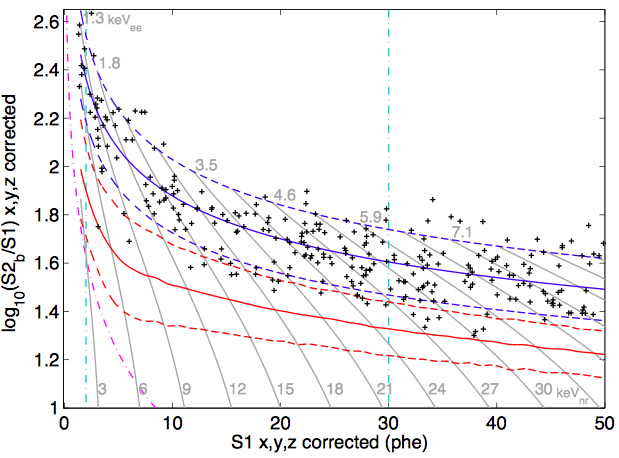
\includegraphics[width=120mm]{Chapter_LUX_Det/LUX_Result.png}
\caption{LUX Result.}
\label{fig:LUX_Result}
\end{figure}

The result from the first science run with the LUX detector is consistent with a P value of 0.35 for the null hypothesis. The 90\% upper C.L. cross section for various spin independent masses are shows in figure \ref{fig:LUX_Limit}. The minimum cross section reported occurs at 7.6$\rm\times10^{-46}$ $\rm cm^2$ for a WIMP mass of 33 GeV/$\rm c^2$. For more detail see [ref LUX PRL].

 \begin{figure}[h!]\centering
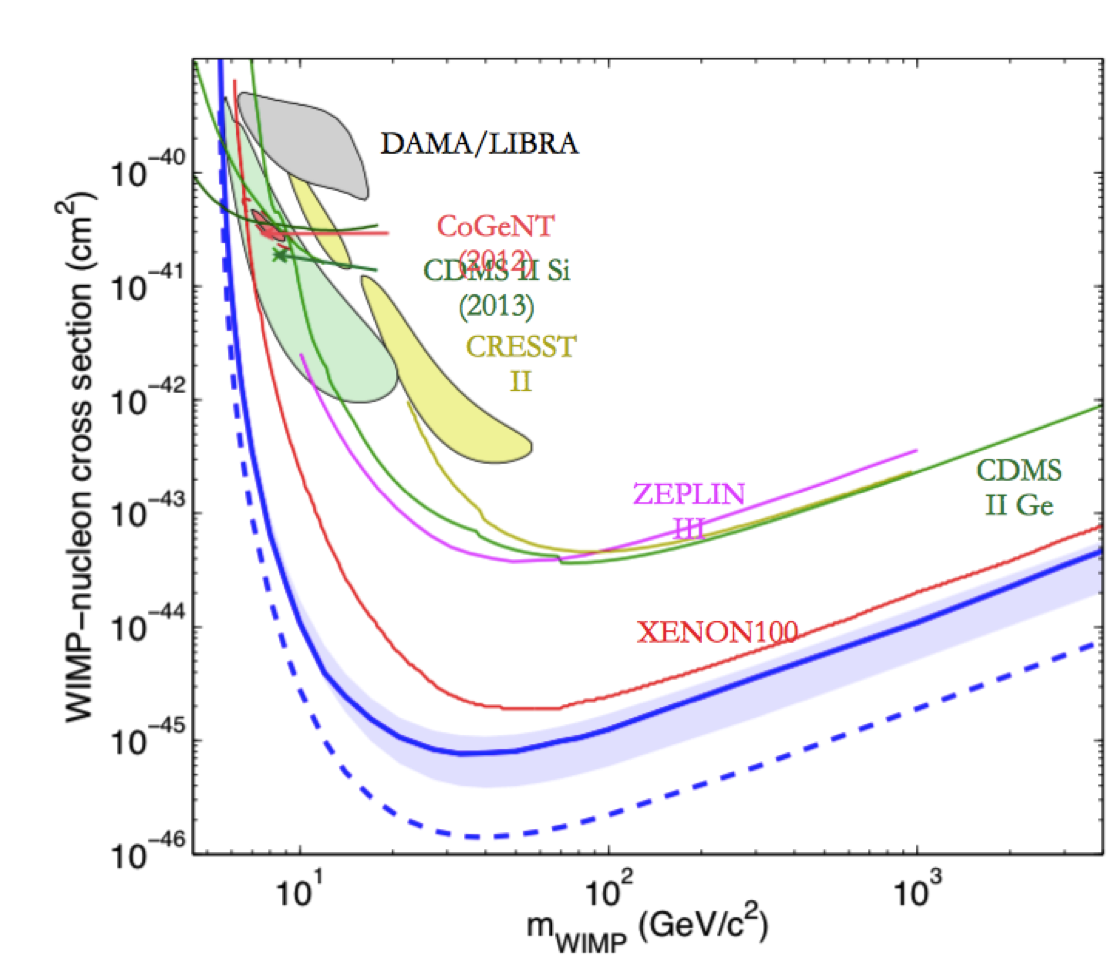
\includegraphics[width=120mm]{Chapter_LUX_Det/LUX_Limit.png}
\caption{LUX WIMP Limit.}
\label{fig:LUX_Limit}
\end{figure}


The ER band used for the first science result was calibrated using a novel tritium source which will be discussed in further detail in this thesis. Since the initial science run we have gathered twenty times the tritium statistics to populate the ER band, with as much as 150,000 in the fiducial. We also spent several months deploying a DD neutron generated source to nail down the NR band mean. The results from the improved ER and NR calibrations will be reported in this thesis along with the implications for an improved WIMP limit. A full reanalysis of the LUX WIMP limit from 2013 will appear in late Fall of 2014. 
